\setchapterpreamble[u]{\margintoc}
\chapter{The Regression Theory of Everything}
\labch{intro}

\textit{"AI Scientists disagree as to whether these language networks posess true knowledge or are just mimicking humans by remembering the statistics of millions of words. I don't believe any kind of deep learning network will achieve the goal of AGI [Artificial General Intelligence] if the network doesn't model the world the way the brain does. Deep learning networks work well, but not because they solved the knowledge representation problem. They work well because they avoided it completely, relying on statistics and lots of data instead. How deep learning networks work is clever, their performance impressive, and they are commercially valuable. I am only pointing out that they don't possess knowledge and, therefore, are not on the path to having the ability of a five-year-old child."} Jeff Hawkins, 2022 \cite{hawkins_2022}

\section{Let's Avoid Knowledge Representation!}

The knowledge representation problem in AI is the challenge of how to formally represent knowledge in a way that a computer can understand and reason about. This typically involves creating a set of symbols, rules, and structures that can be used to represent concepts, relationships, and other types of information. The goal is to create a representation that is both expressive enough to capture all relevant aspects of the domain, and computationally tractable enough to allow for efficient reasoning and inference. There are many different approaches to knowledge representation, including logic-based, semantic networks, frames, and ontologies, each with their own strengths and weaknesses.

Deep learning techniques handle knowledge representation differently than traditional symbolic AI methods. Unlike symbolic AI, which relies on explicit and hand-coded representations of knowledge, deep learning techniques learn to represent knowledge implicitly through the use of neural networks.


\begin{marginfigure}[-5.5cm]
        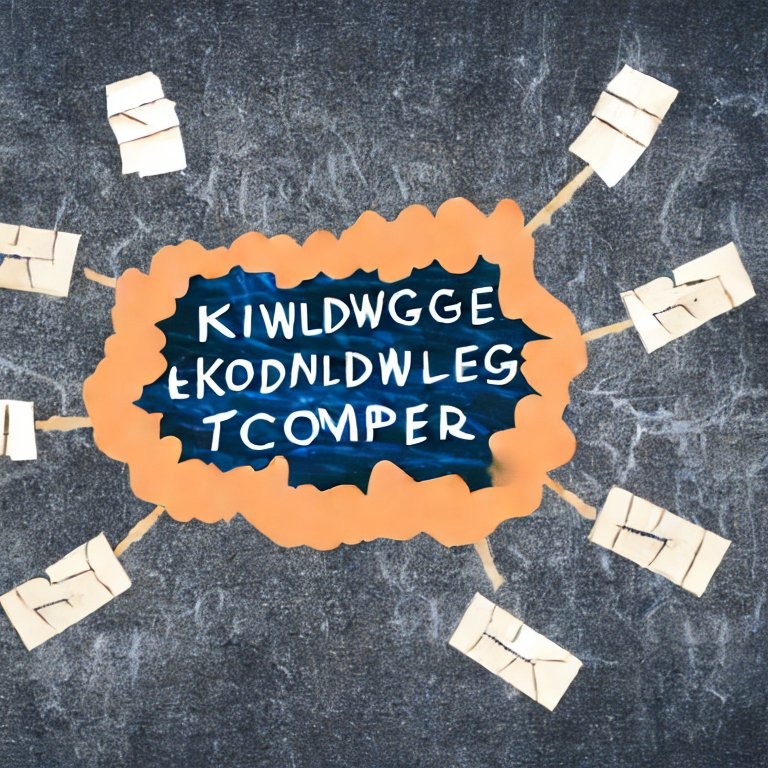
\includegraphics{knowledge}
        \caption{"representing knowledge to a comupter" by Stable Diffusion 2.1}
        \labfig{marginknowledge}
\end{marginfigure}


In deep learning, knowledge is represented in the form of the weights of the neural network. These weights are learned through training on a large dataset and they capture the underlying relationships and patterns in the data. The neural network can then use these learned weights to make predictions, classifications or generate new data.

Deep learning models can handle large and complex datasets, and can automatically extract features from the data without the need for manual feature engineering. This makes them particularly well-suited for tasks such as image and speech recognition, natural language processing, and other areas where large amounts of data are available. However, they are not as good at explicating how they arrived at a decision, which can be a disadvantage.

In summary, deep learning techniques handle knowledge representation by learning the underlying patterns and relationships in the data through the use of neural networks, which can then be used for prediction, classification, and generation tasks.

\section{A Simple Neural Network is also a Linear Regression}

A neural network can be mathematically equivalent to a regression or a decision tree under certain conditions.

A neural network is a machine learning model composed of layers of interconnected artificial neurons, which are designed to process and analyze data. They can be used for a wide range of tasks, such as image and speech recognition, natural language processing, and prediction.

\begin{marginfigure}[-5.5cm]
	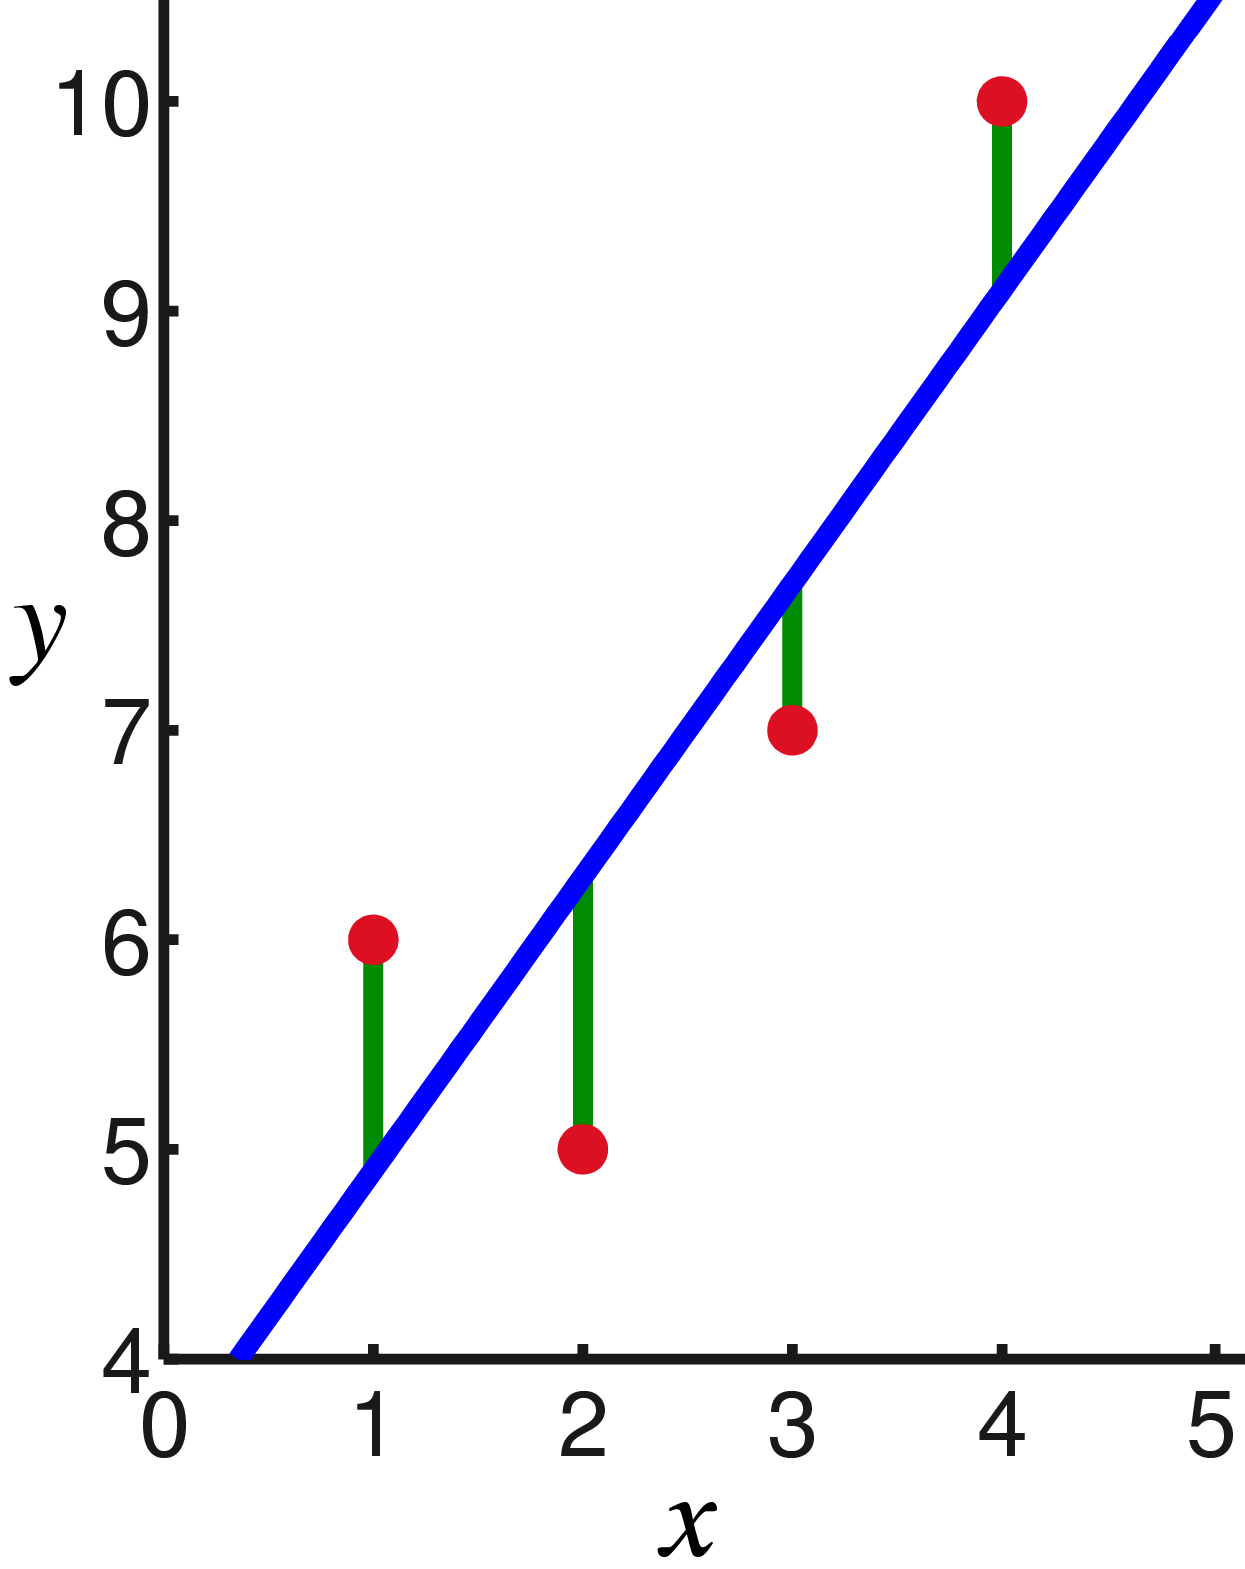
\includegraphics{OLSregression}
        \caption{A simple linear regression, the red points are the training data, and the blue line is the regression line.}
        \labfig{olsregression}
\end{marginfigure}


A regression is a statistical method used to predict a continuous variable based on one or more input features. A linear regression, for example, is a simple neural network with one input layer, one output layer and no hidden layers. In this case, the weights of the network are the coefficients of the linear equation and the network is equivalent to a linear regression model.

A decision tree is a tree-based model used for classification and prediction tasks. It consists of a series of if-then rules that are used to make decisions based on the input data. A neural network with one input layer, one output layer and one hidden layer with the ReLU activation \sidenote{Neurons in a neural network can have different \href{https://en.wikipedia.org/wiki/Activation\_function}{activation functions}, if you don't know what it is and don't want to read about it in wikipedia, that's OK.} function is equivalent to a decision tree. This is because the ReLU activation function allows the network to implement a piecewise linear function which can represent the decision boundaries of a decision tree.

In summary, under certain conditions, a neural network can be mathematically equivalent to a linear regression or a decision tree. These conditions include having one input and one output layers, and having a specific activation function in the case of a decision tree.\sidecite{Aytekin}

\section{Dummy Variables for Dummies (Wonkish)} 

Chapter Summary: It's all numbers, man. Machine learning techniques require that we turn everything (images, text, sound) into numbers and shove them into the model in the same way we use dummy variables in a simple regression. If you are satisfied with this, please skip this section. If you would like to learn a bit about the details and see some code examples, please keep reading. This section is necessarily technical, but should be approachable for anyone who has taken a college statistics class. \sidenote{Thanks to Paul Krugman for popularizing (to me at least) the \textit{wonkish} classifier, I just mean it's a little nerdy. But it's important.} 



Dummy variables are used in regression analysis to include categorical variables in a model. Categorical variables are variables that take on a finite number of distinct values, such as "red", "green", "blue" or "yes", "no". Since these variables cannot be directly included in a regression model, as they are not numerical, they need to be transformed into numerical variables.

The process of creating dummy variables is also known as one-hot encoding. It involves creating a new binary variable for each category of the original variable. For example, if you have a categorical variable "color" with three categories: "red", "green", "blue", you would create three binary variables: "color\_red", "color\_green", "color\_blue". Each binary variable would take a value of 1 if the original variable is equal to the category, and 0 otherwise.

When using dummy variables in a regression, it is important to remember to include only n-1 binary variables, where n is the number of categories in the original variable. This is because including all n binary variables would result in perfect multicollinearity, which is when two or more independent variables are perfectly correlated. One of the binary variables can be dropped to avoid this problem.

Dummy variables are used in regression analysis to include categorical variables in a model. The process of creating dummy variables involves creating a new binary variable for each category of the original variable and one-hot encoding it. It is important to remember to include only n-1 binary variables, to avoid perfect multicollinearity.



\begin{marginlisting}[-0.5cm]
\caption{Mapping text to numbers.}
\vspace{0.2cm}
\begin{lstlisting}[language=Python,style=kaolstplain]
 'movies': 99,
 'after': 100,
 'think': 101,
 'characters': 102,
 'watch': 103,
 'two': 104,
 'films': 105,
 'character': 106,
 'seen': 107,
 'many': 108,
 'being': 109
\end{lstlisting}
\end{marginlisting}


The creation of dummy variables in a regression is analgous to preprocessing image, text and other data for a nueural network for deep learning. This preprocessing is important  as it ensures that the data is in a format that can be easily understood and processed by the network. The preprocessing steps for numbers, text, and images are slightly different.

For numbers:
\begin{itemize}
	\item Normalization: It is common to normalize the input data by scaling it to have a mean of 0 and a standard deviation of 1. This helps to ensure that all input features have similar scales and prevents any one feature from dominating the network's computations.
	\item Imputation: Handling missing data is important, as it can negatively impact the model's performance. Common imputation techniques include replacing missing values with the mean, median, or mode of the feature.
\end{itemize}

For text:

\begin{itemize}
	\item Tokenization: Text data must first be converted into a numerical format that can be understood by the network. This is typically done by tokenizing the text into individual words or n-grams and then encoding them as integers or real-valued vectors. A one-hot encoding exactly like the dummy variable method used in regression is also frequently used. \sidenote{Sometimes text is just mapped to a number! Shocking, but it works. \href{https://www.tensorflow.org/text/guide/word\_embeddings}{Read more about word embeddings in the Tensorflow official tutorials}.} \sidenote{GPT-3 uses byte-level Byte Pair Encoding (BPE) tokenization and has a vocabulary size of 50,257.}
	\item Stop-words removal: The most common words in any language like "a", "an", "the", etc. that do not contain much meaning are called stop-words, they are often removed to reduce the dimensionality of the data.
	\item Stemming/Lemmatization: Words that have the same meaning can be stemmed or lemmatized to reduce the vocabulary size and increase the chances of generalization.
	\item Vocabulary Size: Each model must choose a vocabulary size or the maximum number of tokens that it will analyze. This may cause misspellings, slang or typos to be discarded in analysis.
\end{itemize}

For images:
    
\begin{itemize}
	\item Converting to RGB or Greyscale: Each image is analyzed by its pixel color value, every point on an image will either have 3 color values (red, green, blue) or one single value (on a white/black scale) if the image is analyzed in greyscale.
	\item Convolutions: Pixel values are analyzed in groups that are defined by the model, since individual pixel values are only colors (or greyness) they must be combined together by the model to detect patterns like faces and stop signs. The method of convolution is defined by the model itself.
	\item Resizing: neural network can only accept images of a fixed size, so resizing the image to match the network's requirements is important.
	\item Normalization: It is common to normalize the pixel values to be in the range of 0-1 or -1 to 1. This will help the model converge faster.
	\item Data Augmentation: To increase the amount of data and prevent overfitting, common data augmentation techniques such as flipping, rotation, and cropping can be applied to the images.
\end{itemize}

In summary, preprocessing is an important step in training a neural network, as it ensures that the data is in a format that can be easily understood and processed by the network. The preprocessing steps for numbers, text, and images involve normalization, imputation, tokenization, stop-words removal, stemming/lemmatization, resizing and data augmentation.

\section{Try That Again With 33,640,010 Parameters}

In the first section of this chapter we introduced the idea that a simple neural network is mathematically equivalent to a regression. This is true and a useful way to think about neural networks and deep learning. \sidenote{\begin{equation}y=Wx+b\end{equation} There's your simple formula for a single-cell neural network and regression, in practice we'll change $W$, $x$ and $b$ to matricies and introduce nonlinear activiation function $f$ so, \begin{equation}y=f(Wx+b)\end{equation} if you please. If equations scare you, don't worry about it for now.} 

In practice, neural networks frequently trained with millions of parameters. Here is an example of the trainable parameters of a simple image classifier. This example is a dense neural network to classify handwritten digits, and is not yet as sophisticated as the one used by Yann LeCun and and company in the 1990s

In these next few examples, don't worry if you don't understand the layer types or know what batch nomalization means. The point I would like to make is that neural networks are often created with millions of trainable parameters, once you agree with me regarding this point we will discuss the implications of this in more depth.

\begin{lstlisting}[style=kaolstplain,linewidth=1.5\textwidth]
_________________________________________________________________
Layer (type)                 Output Shape              Param #   
=================================================================
dense (Dense)                (None, 64)                50240     
_________________________________________________________________
batch_normalization (BatchNo (None, 64)                256       
_________________________________________________________________
dense_1 (Dense)              (None, 64)                4160      
_________________________________________________________________
batch_normalization_1 (Batch (None, 64)                256       
_________________________________________________________________
dense_2 (Dense)              (None, 64)                4160      
_________________________________________________________________
batch_normalization_2 (Batch (None, 64)                256       
_________________________________________________________________
dropout (Dropout)            (None, 64)                0         
_________________________________________________________________
dense_3 (Dense)              (None, 10)                650       
=================================================================
Total params: 59,978
Trainable params: 59,594
Non-trainable params: 384
_________________________________________________________________
\end{lstlisting}

59,594 parameters! That's not too bad for a simple neural network, but in practice the networks often get even bigger. Here is a \textit{real} example that will make your brain a little hot.

\begin{lstlisting}[style=kaolstplain,linewidth=1.5\textwidth]
Layer (type)                 Output Shape              Param #   
=================================================================
conv2d (Conv2D)              (None, 28, 28, 64)        640       
_________________________________________________________________
conv2d_1 (Conv2D)            (None, 28, 28, 64)        36928     
_________________________________________________________________
max_pooling2d (MaxPooling2D) (None, 14, 14, 64)        0         
_________________________________________________________________
batch_normalization (BatchNo (None, 14, 14, 64)        256       
_________________________________________________________________
conv2d_2 (Conv2D)            (None, 14, 14, 128)       73856     
_________________________________________________________________
conv2d_3 (Conv2D)            (None, 14, 14, 128)       147584    
_________________________________________________________________
max_pooling2d_1 (MaxPooling2 (None, 7, 7, 128)         0         
_________________________________________________________________
batch_normalization_1 (Batch (None, 7, 7, 128)         512       
_________________________________________________________________
conv2d_4 (Conv2D)            (None, 7, 7, 256)         295168    
_________________________________________________________________
conv2d_5 (Conv2D)            (None, 7, 7, 256)         590080    
_________________________________________________________________
conv2d_6 (Conv2D)            (None, 7, 7, 256)         590080    
_________________________________________________________________
max_pooling2d_2 (MaxPooling2 (None, 3, 3, 256)         0         
_________________________________________________________________
batch_normalization_2 (Batch (None, 3, 3, 256)         1024      
_________________________________________________________________
conv2d_7 (Conv2D)            (None, 3, 3, 512)         1180160   
_________________________________________________________________
conv2d_8 (Conv2D)            (None, 3, 3, 512)         2359808   
_________________________________________________________________
conv2d_9 (Conv2D)            (None, 3, 3, 512)         2359808   
_________________________________________________________________
max_pooling2d_3 (MaxPooling2 (None, 2, 2, 512)         0         
_________________________________________________________________
batch_normalization_3 (Batch (None, 2, 2, 512)         2048      
_________________________________________________________________
conv2d_10 (Conv2D)           (None, 2, 2, 512)         2359808   
_________________________________________________________________
conv2d_11 (Conv2D)           (None, 2, 2, 512)         2359808   
_________________________________________________________________
conv2d_12 (Conv2D)           (None, 2, 2, 512)         2359808   
_________________________________________________________________
max_pooling2d_4 (MaxPooling2 (None, 1, 1, 512)         0         
_________________________________________________________________
batch_normalization_4 (Batch (None, 1, 1, 512)         2048      
_________________________________________________________________
flatten (Flatten)            (None, 512)               0         
_________________________________________________________________
dense (Dense)                (None, 4096)              2101248   
_________________________________________________________________
dropout (Dropout)            (None, 4096)              0         
_________________________________________________________________
dense_1 (Dense)              (None, 4096)              16781312  
_________________________________________________________________
dropout_1 (Dropout)          (None, 4096)              0         
_________________________________________________________________
dense_2 (Dense)              (None, 10)                40970     
=================================================================
Total params: 33,642,954
Trainable params: 33,640,010
Non-trainable params: 2,944
_________________________________________________________________
\end{lstlisting}

When a neural network has millions of trainable parameters and deep layers of neurons, it can be difficult to explain to a human what each of those parameters represents or how they contribute to the overall function of the network. This is because the interactions between the different layers and neurons can be complex and non-linear, making it challenging to understand the specific role of each parameter. Additionally, many of the parameters are used to model complex interactions between the inputs and outputs, making it difficult to understand their specific function. Furthermore, in deep neural networks, the high number of layers can lead to high level of abstraction, meaning that the individual neurons and their weights have little interpretability.

Additionally, when a neural network has millions of interacting parameters, it can lead to mathematical chaos \sidenote{\href{https://en.wikipedia.org/wiki/Chaos_theory}{Mathematical chaos} is a real thing! Mathematical chaos refers to the behavior of certain dynamic systems that are highly sensitive to initial conditions. This sensitivity leads to seemingly random and unpredictable behavior, even though the underlying equations governing the system are deterministic (meaning they are transparent and known to us).}, which is a phenomenon where small changes in the initial conditions of the network can lead to vastly different outputs. This is because the interactions between the large number of parameters can create non-linear relationships that are sensitive to small changes. This can make it difficult to predict the behavior of the network, as small changes in the input or the parameters can lead to unexpected and seemingly random outputs. Additionally, the large number of parameters can make the network more prone to overfitting, where the network is able to memorize the training data but is not able to generalize to new data. This can further exacerbate the problem of chaotic behavior, as the network may produce unpredictable results on new, unseen data.

\section{Multicolinearity and the End of Science}

\section{Let's Test Some Random Inputs! Feature Importance and Explainability}

\section{The Universal Machine Learning Workflow}

Summarize and opine on The Universal Machine Learning Workflow \sidecite{chollet_2022}
